\documentclass[11pt]{article}
\usepackage{graphicx}
\usepackage[bookmarks=true]{hyperref}
\usepackage{bookmark}
\usepackage{hyperref}
\usepackage{csquotes}
\usepackage{float}
\usepackage{wrapfig}
\usepackage[normalem]{ulem}
\useunder{\uline}{\ul}{}

\usepackage{array}
\newcolumntype{L}[1]{>{\raggedright\let\newline\\\arraybackslash\hspace{0pt}}m{#1}}
\newcolumntype{C}[1]{>{\centering\let\newline\\\arraybackslash\hspace{0pt}}m{#1}}
\newcolumntype{R}[1]{>{\raggedleft\let\newline\\\arraybackslash\hspace{0pt}}m{#1}}

\setlength{\parindent}{0pt}

\begin{document}

\begin{titlepage}
\begin{flushright}


\includegraphics[width=380px]{../global/University_of_Pretoria_Logo.png}
\newline
\newline

\textbf {\LARGE Plan for Software Aspects of Certification} \newline

\textbf {\Large (PSAC)} \newline

\centering
\includegraphics[width=100px]{../global/Logo.jpg}

\textbf {\Large Linphone for Android Group Chat (Waterfall)}\newline

\flushright \textbf {\large Version: 1.2}\newline

\centering \textbf {\large Authors:}

\begin{table}[H]
\large
\centering
\begin{tabular}{rl}
	Izak Blom & 13126777 \\
	David Breetzke & 12056503 \\
	Paul Engelke & 13093500 \\
	Prenolan Govender & 13102380 \\
	Jessica Lessev & 13049136 \\
\end{tabular}
\end{table}

Date: \today

\end{flushright}
\end{titlepage}

\setcounter{tocdepth}{3}
\setcounter{secnumdepth}{5}
\tableofcontents

\newpage
\section{Revision History}
\begin{table}[h]
\begin{tabular}{llll}
\textbf{Date}          & \textbf{Description}  & \textbf{Author}       & \textbf{Comments}   \\ \hline
\multicolumn{1}{|R{2cm}|}{23/06/2015} & \multicolumn{1}{L{4.5cm}|}{Document Creation} & \multicolumn{1}{l|}{Team Eclectic} & \multicolumn{1}{L{4cm}|}{Version 1} \\ \hline
\multicolumn{1}{|l|}{} & \multicolumn{1}{l|}{} & \multicolumn{1}{l|}{} & \multicolumn{1}{l|}{} \\ \hline
\multicolumn{1}{|l|}{} & \multicolumn{1}{l|}{} & \multicolumn{1}{l|}{} & \multicolumn{1}{l|}{} \\ \hline
\multicolumn{1}{|l|}{} & \multicolumn{1}{l|}{} & \multicolumn{1}{l|}{} & \multicolumn{1}{l|}{} \\ \hline
\multicolumn{1}{|l|}{} & \multicolumn{1}{l|}{} & \multicolumn{1}{l|}{} & \multicolumn{1}{l|}{} \\ \hline
\multicolumn{1}{|l|}{} & \multicolumn{1}{l|}{} & \multicolumn{1}{l|}{} & \multicolumn{1}{l|}{} \\ \hline
\multicolumn{1}{|l|}{} & \multicolumn{1}{l|}{} & \multicolumn{1}{l|}{} & \multicolumn{1}{l|}{} \\ \hline
\multicolumn{1}{|l|}{} & \multicolumn{1}{l|}{} & \multicolumn{1}{l|}{} & \multicolumn{1}{l|}{} \\ \hline
\multicolumn{1}{|l|}{} & \multicolumn{1}{l|}{} & \multicolumn{1}{l|}{} & \multicolumn{1}{l|}{} \\ \hline
\multicolumn{1}{|l|}{} & \multicolumn{1}{l|}{} & \multicolumn{1}{l|}{} & \multicolumn{1}{l|}{} \\ \hline
\multicolumn{1}{|l|}{} & \multicolumn{1}{l|}{} & \multicolumn{1}{l|}{} & \multicolumn{1}{l|}{} \\ \hline
\multicolumn{1}{|l|}{} & \multicolumn{1}{l|}{} & \multicolumn{1}{l|}{} & \multicolumn{1}{l|}{} \\ \hline
\multicolumn{1}{|l|}{} & \multicolumn{1}{l|}{} & \multicolumn{1}{l|}{} & \multicolumn{1}{l|}{} \\ \hline
\multicolumn{1}{|l|}{} & \multicolumn{1}{l|}{} & \multicolumn{1}{l|}{} & \multicolumn{1}{l|}{} \\ \hline
\multicolumn{1}{|l|}{} & \multicolumn{1}{l|}{} & \multicolumn{1}{l|}{} & \multicolumn{1}{l|}{} \\ \hline
\end{tabular}
\end{table}

\section{Document Approval}
\begin{table}[h]
\begin{tabular}{llll}
\textbf{Signature}     & \textbf{Printed Name} & \textbf{Title}        & \textbf{Comments}     \\ \hline
\multicolumn{1}{|l|}{} & \multicolumn{1}{L{3.5cm}|}{} & \multicolumn{1}{L{3.5cm}|}{} & \multicolumn{1}{L{4cm}|}{} \\ \hline
\multicolumn{1}{|l|}{} & \multicolumn{1}{l|}{} & \multicolumn{1}{l|}{} & \multicolumn{1}{l|}{} \\ \hline
\multicolumn{1}{|l|}{} & \multicolumn{1}{l|}{} & \multicolumn{1}{l|}{} & \multicolumn{1}{l|}{} \\ \hline
\multicolumn{1}{|l|}{} & \multicolumn{1}{l|}{} & \multicolumn{1}{l|}{} & \multicolumn{1}{l|}{} \\ \hline
\end{tabular}
\end{table}

\newpage
\section{Introduction}
\subsection{Document Scope}
This document discusses the design choices and implementation for the Linphone Group Chat extension. The document introduces a number of new classes and interfaces as well as changes to existing code. Low-level implementation design and logic flow are also discussed.
\subsection{Acronyms}
\begin{itemize}
\item \textbf{SRS} Software Requirements Specification
\item \textbf{SDD} Software Design Description
\item \textbf{AES256} Advanced Encryption Standard (256-bit)
\end{itemize}
\section{Classes \& Interfaces}
\subsection{Interfaces}
This section discusses new interfaces, listed in alphabetical order.
\subsubsection{EncryptionHandler}
The \textit{EncryptionHandler} interface defines how interaction with an \textit{EncryptionHandler} implementation takes place. An encryption handler will be used by a \textit{ \hyperref[subsubsec: linphonegroupchatroom]{LinphoneGroupChatRoom}} instance to perform the necessary encryption/decryption operations.\\
This interface and its implementing classes fulfil certain requirements specified in the \textbf{Software Requirements Specification} document, specifically those pertaining to encryption and message security.
\begin{figure}[H]
\centering
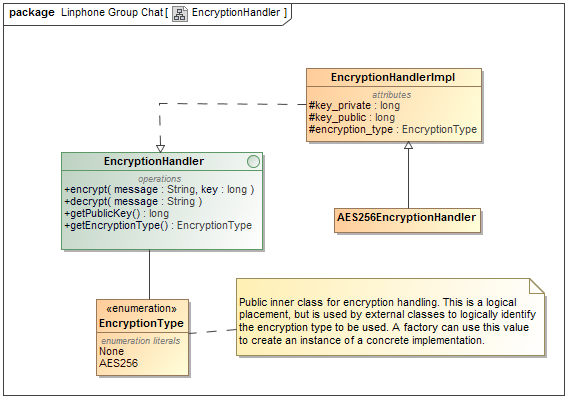
\includegraphics[width=5in]{./images/class_encryption_handler.png}
\caption[EncrpytionHandler Class Diagram]{This diagram shows the operations available in the \textit{EncryptionHandler} interface and the classes that implement it.}
\label{cd-encryption-handler}
\end{figure}
\subsubsection{EncryptionStrategy}
The \textit{EncryptionStrategy} interface describes how a \textit{ \hyperref[subsubsec: linphonegroupchatroom]{LinphoneGroupChatRoom}} instance will interact with the \textit{EncryptionStrategy} implementation. The motivation for using a strategy is that the code for an implementation that does not use encryption and one that does, may vary significantly. Using a strategy, we might reduce boiler-plate code and promote loose coupling between the \textit{LinphoneGroupChatRoom} instance and the encryption algorithm, if any.
\begin{figure}[H]
\centering
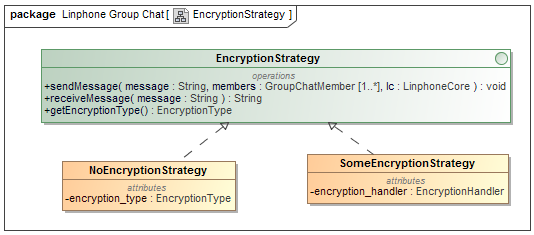
\includegraphics[width=5in]{./images/class_encryption_strategy.png}
\caption[EncryptionStrategy Class Diagram]{A class diagram showing the \textit{EncryptionStrategy} interface and implementing classes.}
\label{cd-encryption-strategy}
\end{figure}
\subsubsection{GroupChatStorage}
The \textit{GroupChatStorage} interface defines how interaction between the persistence tool and a \textit{ \hyperref[subsubsec: linphonegroupchatroom]{LinphoneGroupChatRoom}} instance takes place.\\
This interface accommodates for certain requirements specified in the \textbf{Software Requirements Specification}. These include, among others, message status indications (received/sent/pending) and local message deletion.
\begin{figure}[H]
\centering
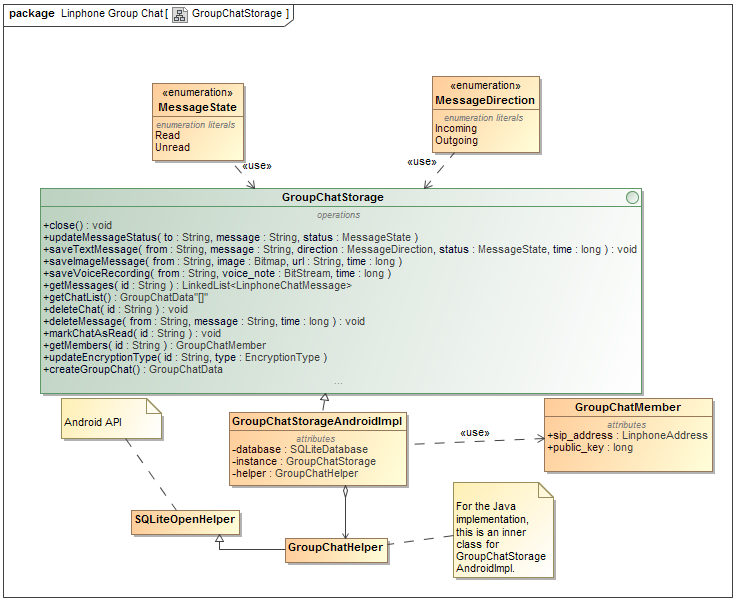
\includegraphics[width=5in]{./images/class_chat_storage.png}
\caption[GroupChatStorage Class Diagram]{This diagram describes the GroupChatStorage interface.}
\label{cd-chat-storage}
\end{figure}
\subsection{Linphone Group Chat: Core Classes}
This section discusses new class implementations, listed in alphabetical order.
\subsubsection{AES256EncryptionHandler}
The \textit{AES256EncryptionHandler} performs AES256 encryption and decryption on strings.\\
The class diagram can be seen in figure \ref{cd-encryption-handler}.
\subsubsection{EncryptionHandlerImpl}
The \textit{EncryptionHandlerImpl} class is an abstract class that provides certain basic attributes necessary for encryption. This class can be extended for more concrete implementations using different encryption algorithms.\\
The class diagram can be seen in figure \ref{cd-encryption-handler}.
\subsubsection{GroupChatStorageAndroidImpl}
The \textit{GroupChatStorageAndroidImpl} implements the \textit{GroupChatStorage} interface for android devices. This implementation will allow data related to a \textit{LinphoneGroupChatRoom} to be persisted for reuse.\\
This class will be implemented as a singleton so that the same database connection can be maintained for all group chat instances.\\
The class diagram can be viewed in figure \ref{cd-chat-storage}.\\
\subsubsection{LinphoneGroupChatListener}
The \textit{LinphoneGroupChatListener} implements the \textit{LinphoneCoreListener} interface and is responsible for ensuring that messages intended for group chats are intercepted and deferred to the \textit{LinphoneGroupChatManager} instance. \\
The class is referred to in figure \ref{cd-chat-manager}.
\subsubsection{LinphoneGroupChatManager}
The \textit{LinphoneGroupChatManager} is responsible for handling the creation and deletion of group chat instances, messages handling for group chats, and various other administrative functions.
\begin{figure}[H]
	\centering
	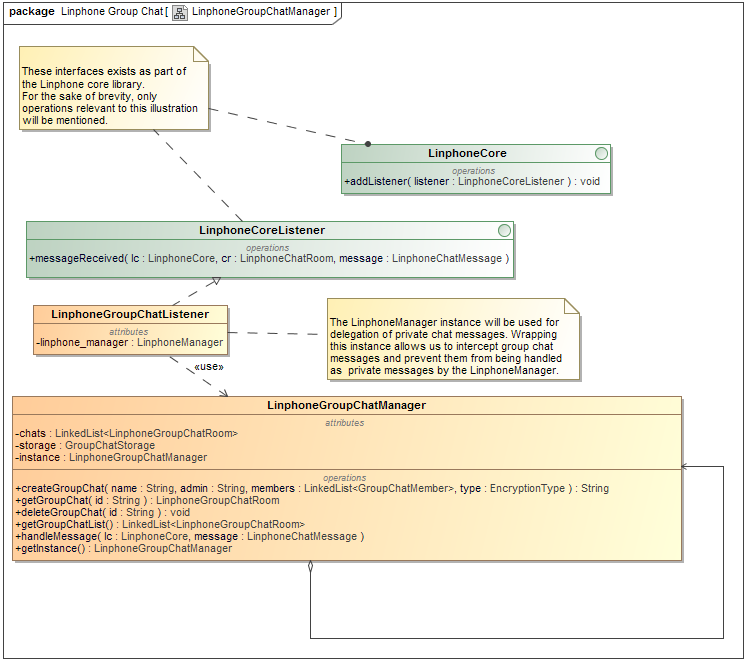
\includegraphics[width=5in]{./images/class_chat_manager.png}
	\caption[LinphoneGroupChatManager Class Diagram]{This diagram depicts the \textit{LinphoneGroupChatManager} class and the relations between relevant classes and interfaces.}
	\label{cd-chat-manager}
\end{figure}
The \textit{LinphoneGroupChatManager} helps realise the requirements and use cases specified in the \textbf{Software Requirements Specification} pertaining to group creation and management.
\subsubsection{LinphoneGroupChatRoom}\label{subsubsec: linphonegroupchatroom}
The \textit{LinphoneGroupChatRoom} class implements the \textit{LinphoneChatRoom} interface with added functionality. The purpose of this class is implement the core workings of a group chat instance, including the management of the group appearance(group name and group picture), group members(adding and removing members) and security(encryption).\\
This class will make use of \textit{LinphoneChatRoomImpl} instances to communicate with each of the group members.
\begin{figure}[H]
\centering
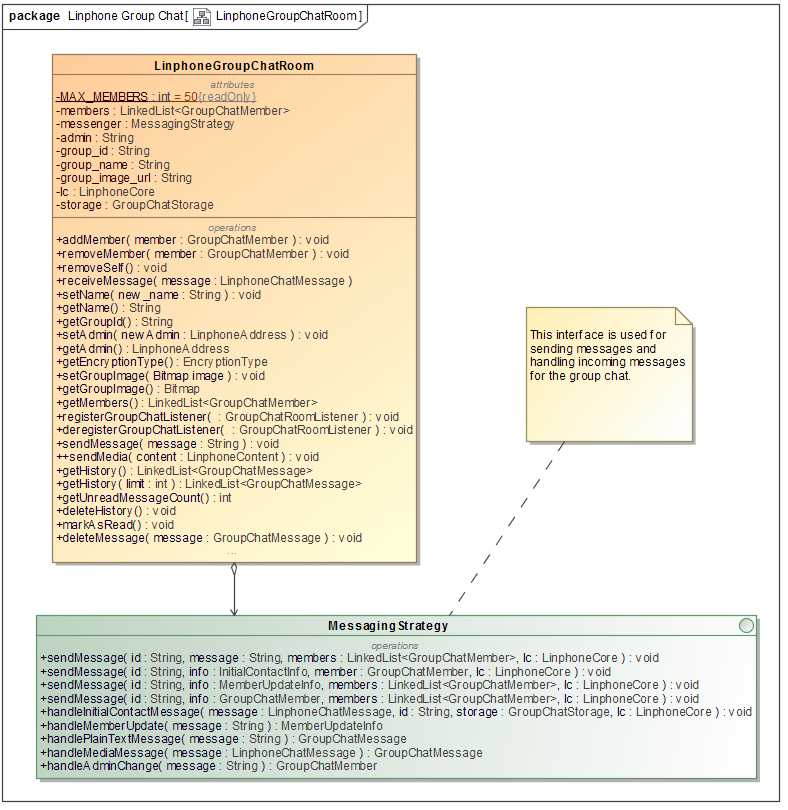
\includegraphics[width=5in]{./images/class_group_chat.png}
\caption[LinphoneGroupChatRoom Clas Diagram]{This diagram shows the implementation design for the \textit{LinphoneGroupChatRoom} class along with relevant relationships with other classes and interfaces.}
\label{cd-group-chat}
\end{figure}
This class helps realise and address the requirements pertaining to group management, such as adding and removing members, addressing the limitations of group sizes and dealing with the security issues of sending and receiving messages. Details on these requirements can be found in the \textbf{Software Requirements Specification} and specific reference can be found in the traceability matrix in Section \ref{section-trace-matrix}.
\subsubsection{NoEncryptionStrategy}
This class implements the \textit{EncryptionStrategy} interface. It defines how a \textit{LinphoneGroupChatRoom} instance will handle sending and receiving messages where no encryption is used. \\
This class can be seen in figure \ref{cd-encryption-strategy}.
\subsubsection{SomeEncryptionStrategy}
This class implements the \textit{EncryptionStrategy} interface. It defines how a \textit{LinphoneGroupChatRoom} instance will handle sending and receiving messages in the presence of an encryption algorithm. At present, this class will encapsulate an \textit{EncryptionHandler} implementation for encryption purposes.
This class can be seen in figure \ref{cd-encryption-strategy}.

\subsection{Linphone Group Chat: Android Classes}
This section lists and describes a number of classes that extend Android specific implementations for the application, specifically the user interface components. The classes are listed in alphabetical order.
\subsubsection{GroupChatActivity}\label{subsubsec: groupchatactivity}
The purpose of the \textit{GroupChatAcitivity} class is to provide all the functionality provided by ChatActivity as well as managing user interface views by activating fragments such as \textit{GroupChatMessagingFragment}, which is a specialisation of \textit{ChatFragment} as well as \textit{GroupChatSettingsFragment}. The \textit{GroupChatMessagingFragment} will host the interface for messaging and the \textit{GroupChatSettingsFragment} will host the interface for manipulation of group-chat settings. This class can be seen in figure ~\ref{cd-group-chat-messaging-ui}.
\subsubsection{GroupChatMessageAdapter}
The \textit{GroupChatMessageAdapter} will retrieve chat history for the \textit{GroupChatMessagingFragment} so that it can be added to the user interface as clearly separated message bubbles. Each message in the chat history will be converted to a message bubble and added to the \textit{GroupChatMessagingFragment}, which adds it to the displayed user interface. This class can be seen in figure ~\ref{cd-group-chat-messaging-ui}.
\subsubsection{GroupChatMessagingFragment}
Similar to the existing \textit{ChatFragment}, but there needs to be a reference to \textit{ \hyperref[subsubsec: linphonegroupchatroom]{LinphoneGroupChatRoom}} which will be a specialisation of the exisiting \textit{LinphoneChatRoom}. Send/Receive requests etc. will be delegated to this LinphoneGroupChatRoom instance instead of a \textit{LinphoneChatRoom} instance. Additional attributes required for group-chat messaging will also be defined in the \textit{GroupChatMessagingFragment} class. 
The \textit{GroupChatMessagingFragment} will host the interface for messaging; i.e. sent or received messages will be displayed here in separate message bubbles along with the group name, group image, a text-box for typing messages, a send-message button, a send-image button and a back button to return to the ChatListing page.
This class can be seen in figure ~\ref{cd-group-chat-messaging-ui}.
\begin{figure}[H]
\centering
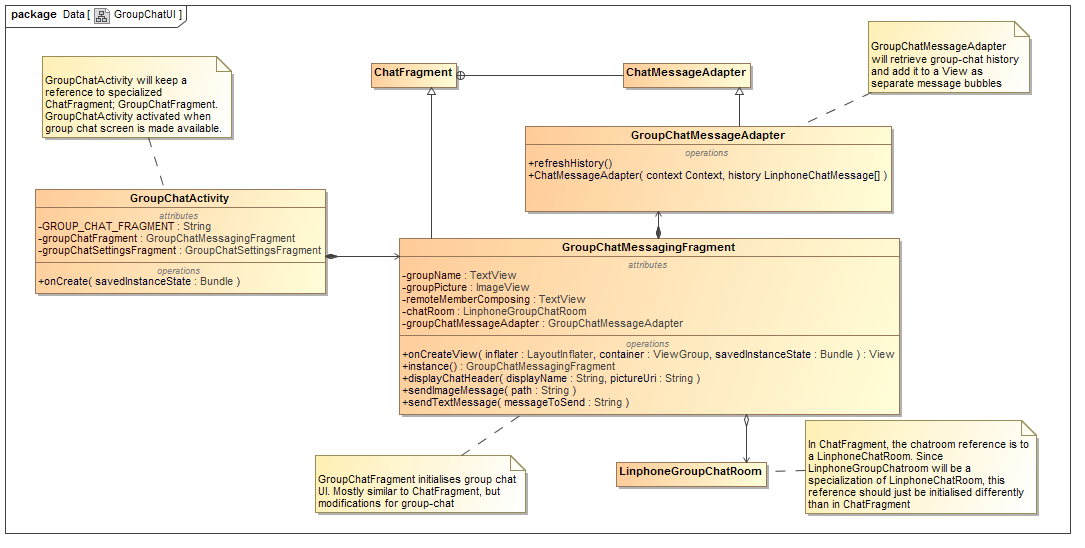
\includegraphics[width=5in]{./images/class_group_chat_messaging_ui.png}
\caption[Android Group Chat Messaging UI Class Diagram]{This diagram shows the implementation design for the \textit{GroupChatActivity}, \textit{GroupChatMessagingFragment} and \textit{GroupChatMessageAdapter} classes along with relevant relationships with other classes and interfaces.}
\label{cd-group-chat-messaging-ui}
\end{figure}
\subsubsection{GroupChatSettingsFragment}
This fragment is contained by a \textit{ \hyperref[subsubsec: groupchatactivity]{GroupChatActivity}} instance and provides the user interface for group-chat settings manipulation. The fragment (and it's associated user interface view) is activated when the user clicks the group-name displayed in \textit{GroupChatMessagingFragment}. The \textit{GroupChatActivity} class manages this fragment along with the \textit{GroupChatMessagingFragment}. This class can be seen in figure ~\ref{cd-group-chat-settings-ui}.
\begin{figure}[H]
\centering
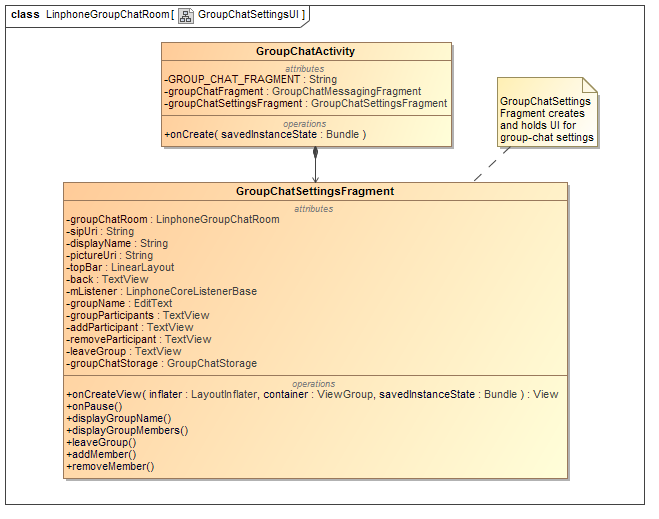
\includegraphics[width=5in]{./images/class_group_chat_settings_ui.png}
\caption[Android Group Chat Settings UI Class Diagram]{This diagram shows the implementation design for the \textit{GroupChatActivity} and \textit{GroupChatSettingsFragment} classes along with relevant relationships with other classes and interfaces.}
\label{cd-group-chat-settings-ui}
\end{figure}
\subsubsection{GroupChatCreationFragment}
This fragment will be contained by a \textit{LinphoneActivity} instance, which is part of the existing Android implementation. The fragment initialises and provides the user interface for group-chat creation. The fragment (and its associated user interface view) is activated when the user clicks on the create-group-chat button to be added to the ChatListing screen. This class can be seen in figure ~\ref{cd-group-chat-creation-ui}.
\begin{figure}[H]
\centering
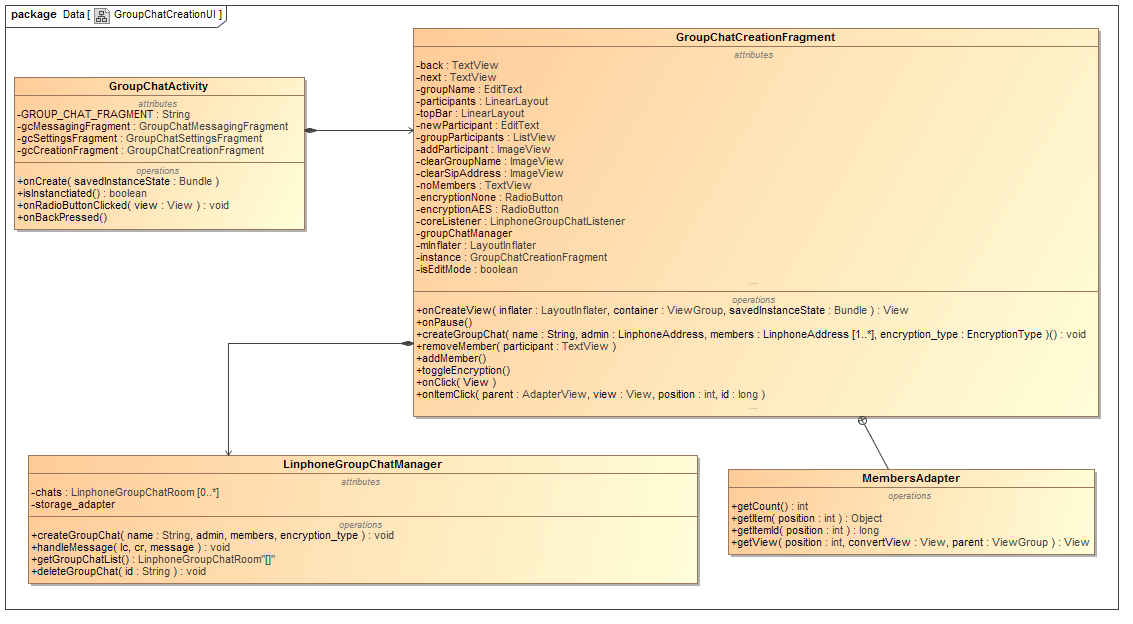
\includegraphics[width=5in]{./images/class_groupchat_creation_ui.png}
\caption[Android Group Chat Creation UI Class Diagram]{This diagram shows the implementation design for the \textit{GroupChatCreationFragment} class along with relevant relationships with other classes and interfaces.}
\label{cd-group-chat-creation-ui}
\end{figure}

\subsection{Modifications To Existing Software}
The Linphone Group Chat extension will form a separate package from the rest of the Linphone source code to simplify the implementation process. When the time comes for integration, certain changes to the existing code will be made to incorporate the new code. Any classes that have been identified, where changes are sure to take place, are listed and briefly discussed below.
\begin{itemize}
\item \textbf{LinphoneManager}\\
This class is responsible for the management of the low-level \textit{Liblinphone} functionality. It's responsibilities include starting the C \textit{Liblinphone} services, reacting to changes in the state of these services and notifying the Android application of these state changes. It also handles notifications for the application that get communicated to the Android system as well as some SIP functionality.\\
This class will wrap itself in a \textit{LinphoneGroupChatListener} instance and initialize the \textit{LinphoneGroupChatManager} instance. The \textit{LinphoneGroupChatListener} will be registered as the \textit{LinphoneCoreListener} for the \textit{LinphoneCore} instance.
\item \textbf{ChatListFragment}\\
This class forms part of the Linphone Android user interface. It initialises and manages the chat-list view, reached when clicking on the chat button located on the bottom navigation bar of the linphone application. In order to create a new group chat, an additional button will be added to this implementation and relative listeners for it will be implemented as well inside the ChatListFragment class. The functionality to list group-chats will also be implemented here. Refer to figure ~\ref{cd-cg} for an illustration of interface modifications mentioned.

\end{itemize}

\section{User Interface Design}
\subsection{Current Interface}
\subsubsection{Linphone interface}
When a Linphone user opens the application, he/she is greeted and interacts with the following interface:
\begin{itemize}
\item	Light shades of blue/grey, dark grey and orange are used as a colour scheme
\item	The user options are located at the bottom of the screen, represented by self-explanatory symbols with an accompanying label.
\item	The user can navigate between these options depending on the needed functionality.
\end{itemize}

\subsubsection{Chat Interface}
The current default interface for a chat between two Linphone users consists of:
\begin{itemize}
\item	A plain blue/grey background
\item	The name of the contact to which the user is currently chatting to is displayed at the top of the chat along with their profile picture.
\subitem Thus functionality will be provided for users to change and update their profile pictures.
\begin{figure}[H]
\centering
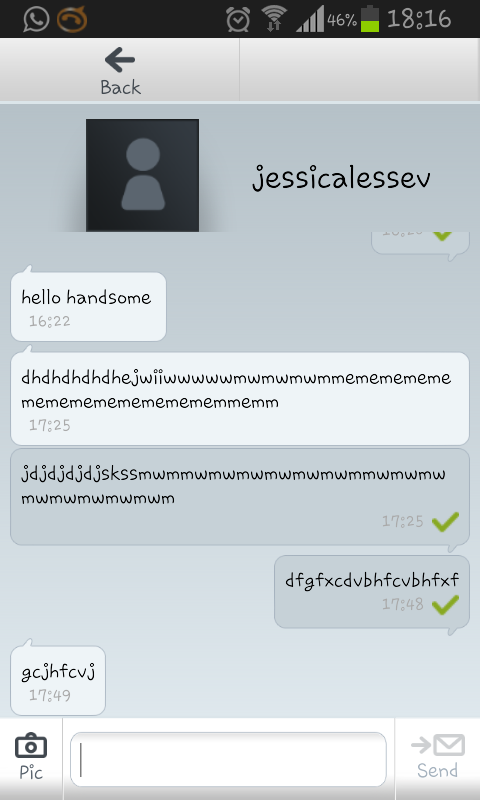
\includegraphics[width=2in]{./images/screen.png}
\caption[Sample Chat Screen]{This diagram shows the current user interface for a chat between two users.}
\label{cd-chat-interface}
\end{figure}
\item	Speech bubbles to represent messages
\subitem	Each speech bubble is either left or right aligned depending on whether it is a the users sent message or the users received message.
\subitem	- A received message appears to be left aligned
\subitem	- A message sent by the user appears to be right aligned
\subitem	- All Speech bubbles representing received messages are represented by a light shade of blue
\subitem	- All speech bubbles representing the users' sent messages are represented by a darker shade of blue.
\item	A yellow arrow represents a sending message
\item	A green tick represents a sent and delivered message
\item	A red cross symbolizes a message that cannot be sent and thus not delivered
\item	When the contact to which the user is chatting to types, the line “Remote is writing…” appears at the bottom of the chat screen

\end{itemize}

\subsubsection{Potential upgrades and changes to Current interface}.\newline
When looking at the current interface that Linphone, from a programmer's perspective, there are some immediate user interface issues that are noticeable, and that can be changed to accommodate the user better. However after comparing several social networking services, such as Skype, Whatsapp, iMessage, BBM etc, many patterns and standards were identified, answering to layout, presentation, and access to functions and options. To further assist with decision making and changes to be made to the user interface, several users were asked to play around with the application and suggest what they like and do not like about the interface, as well as any additional features and changes that could be made to the interface.\\\\
Applying these noted patterns and standards along with the feedback collected from the few users, the following changes to the interface seem plausible: \\\\
Starting from left to right, looking at each screen/option located on the bottom of the menu on the Linphone application:
\paragraph{History Screen}
\begin{itemize}
\item On the top of the screen it is unclear which option is selected between "All" and "Missed" calls. To fix this issue the slider, to indicate the selected option, will be changed to highlight the currently selected option and possibly dim out the unselected option.
\end{itemize}

\paragraph{Contacts Screen}
\begin{itemize}
\item On the top of the screen it is unclear which option is selected between "All" and "SIP" contacts. To fix this issue the slider, to indicate the selected option, will be changed to highlight the currently selected option and possibly dim out the unselected option.

\item On the right to the text box, where one would type to search for a contact, the clear button appears as a small white cross in a red circle. This is so even if the user has not typed anything in the search box. The red circle will appear grey or a faded colour until the user types something in the search box after which the circle can return to its original red colour. 

\item When one is typing in the search bar the text as entered will appear to be left-aligned.
\end{itemize}

\paragraph{Main/Dial Screen}
\begin{itemize}
\item No noticeable interface problems appear on this menu option.
\end{itemize}

\paragraph{Chat Screen}
\begin{itemize}
\item	When one selects the text box to search for a chat the 'place-holder' will disappear and the cursor should be left-aligned.

\item When one is typing in the search bar the text as entered will appear to be left-aligned.

\item On the right to the text box, where one would type to search for a chat, the clear button appears as a small white cross in a red circle. This is so even if the user has not typed anything in the search box. The red circle will appear grey or a faded colour until the user types something in the search box after which the circle can return to its original red colour. 

\item The spacing between the search bar and the first chat in the list will be increased.

\item The display of each chat in the list will change to the following format:
\subitem The name of the contact will appear on the first line - left-aligned.
\subitem The time stamp of the last received message will appear on the first line, right-aligned.
\subitem The last received or sent message will appear on the second line. This will allow for easy location of a chat and easy reading.
\end{itemize}
\paragraph{Within a Chat}
\begin{itemize}
\item A	fine line appears to the right of the "Back" option - since there is not other option to the right this line is useless and will be removed and only added if further options are added to the right of the "Back" button.

\item	Add a defined panel/ bar at the top of a chat to represent the contact to which the user is chatting to. 

\item	Left align the contact details such as picture and name.

\item When one selects the keyboard to type a message the contact's name to which they are talking to changes format. This will not occur and the panel will be kept standard as mentioned in the previous point.

\item	Change the colours of the speech bubbles that represent the messages to be more distinguishable to the background.

\subitem	- The default colour of the speech bubble representing a users' sent message is very similar to the default background colour and thus it is difficult to distinguish the message from the background. Therefore changing the colour of this will allow the messages to stand out and improve visibility of a message.
\subitem 	- The users' sent messages will be represented by a duller colour to the received messages as the received messages need more focus.

\item	Limit the size of speech bubbles.
\subitem - Speech bubbles representing a users' sent message will be limited to stretch to 80\% - 90\% of the screen while being right-aligned.
\subitem	- Speech bubbles representing a received message will be limited to stretch to 80\% - 90\% of the screen while being left-aligned. 
\subitem	- This will allow easier distinguish-ability between sent and received messages when dealing with longer messages.
\subitem	- Improving on the location, direction and size of speech bubbles will provide for a better feedback system.
\begin{figure}[H]
\centering
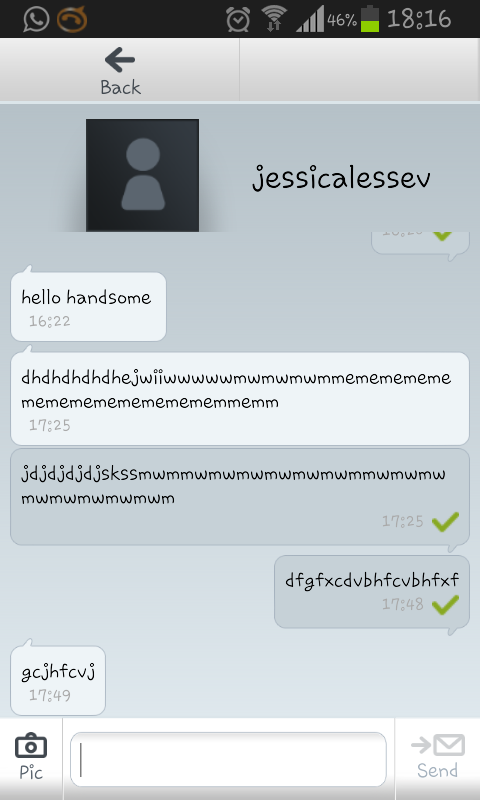
\includegraphics[width=2in]{./images/screen.png}
\caption[Sample Chat Screen]{This diagram shows the current user interface for a chat between two users.}
\label{cd-chat-interface-2}
\end{figure}

\item	The font size of messages will be made larger.

\item	The spacing between words in a messages will be made larger.
\end{itemize}

\paragraph{Settings Screen}
\begin{itemize}
\item No noticeable interface problems appear on this menu option.
\end{itemize}

\subsection{Group Chat Interface}
\subsubsection{Design}
\begin{figure}[H]
\centering
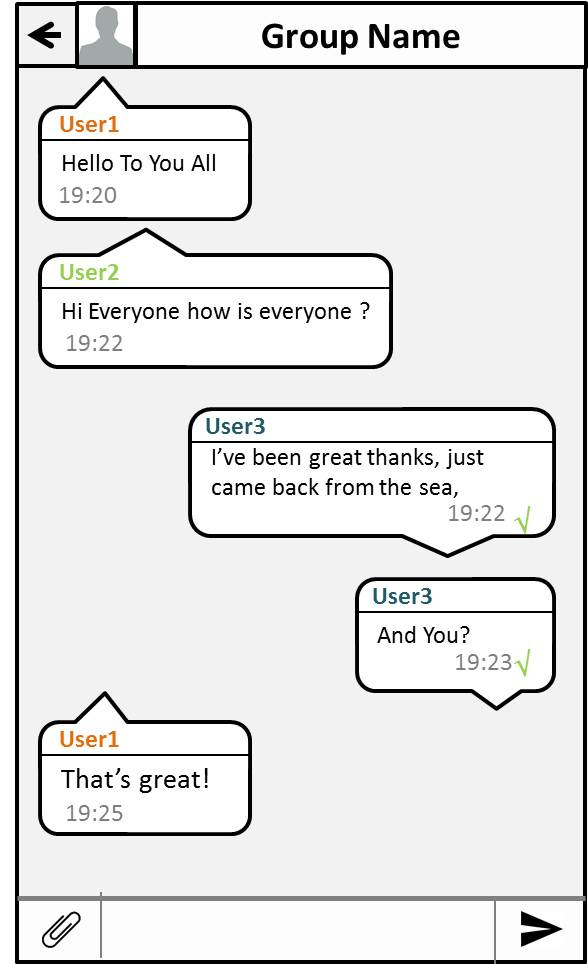
\includegraphics[width=2in]{./images/Final.jpg}
\caption[Sample Group Chat Screen]{This diagram shows how the group chat interface is intended to look.}
\label{cd-group-chat-interface}
\end{figure}

\paragraph{Colours}
\begin{itemize}
\item	In order to maintain consistency of design, the same colours chosen to represent the speech bubble and background throughout the application will be used for the user interface for group chats.
\item	Within each speech bubble, each participant's name will appear in a different colour respectively thus to easily recognize which message came from which participant.
\item	The colour of the text will remain standard.
\item The timestamp will be a light grey and will appear at the bottom left of the received  messages and on the bottom right of the sent messages.
\item The notification symbols such as the cross and tick to indicate the status of the message will remain their default colours.\\
\end{itemize}

\paragraph{Font}
\begin{itemize}
\item	In order to maintain consistency of design, the font size for each message will be the same as the chosen font size for individual chats.
\item The spacing between text will be adjusted to accommodate reading best.
\item	The size of the speech bubbles will again be limited to 80\% - 90\% of the screen to delineate the sender of each message. \\
\end{itemize}

\paragraph{Size}
\begin{itemize}
\item	In order to maintain consistency of design, the font size for each message will be the same as the chosen font size for individual chats.
\item	The size of the speech bubbles will again be limited to 80\% - 90\% of the screen to delineate the sender of each message. \\
\end{itemize}

\paragraph{Speech/Message Bubbles}
\begin{itemize}
\item	Each user will have a uniquely coloured name to represent their message.
\item	The user sending a message will have their speech bubbles appear on the right such as “User 3” in the above diagram
\item	Each participant in the group, not being the main user will have their message bubbles appear on the left – such as user 1 and 2 in the above diagram.
\item Each message bubble will contain a time stamp that will indicate when the message was sent or received.
\item Sent messages from the user will contain a red cross, yellow or green tick depending on whether the message failed to deliver/send, is sending or sent respectively.\\
\end{itemize}

\paragraph{Space}
\begin{itemize}
\item	Moving the group name and picture to appear in the same panel as the "Back" button will allow for more chat space thus more space and less cluttered interface.
\end{itemize}

\paragraph{Icons}
\begin{itemize}
\item	The send icon will be changed to a paper aeroplane symbol.  
\item Since more than one type of media will be able to be sent as a message, the "Image" icon, to represent sending a picture will be replaced by a paper clip icon with the option to send images and voice notes. 
\item The "Back" button will be replaced by a plain standard arrow to symbolize the "Back" option.  
\end{itemize}

\paragraph{Participants}
\begin{itemize}
\item	When the group name is selected a list of the participants will appear.
\end{itemize}


\subsubsection{Group Chat Information}
\begin{figure}[H]
\centering
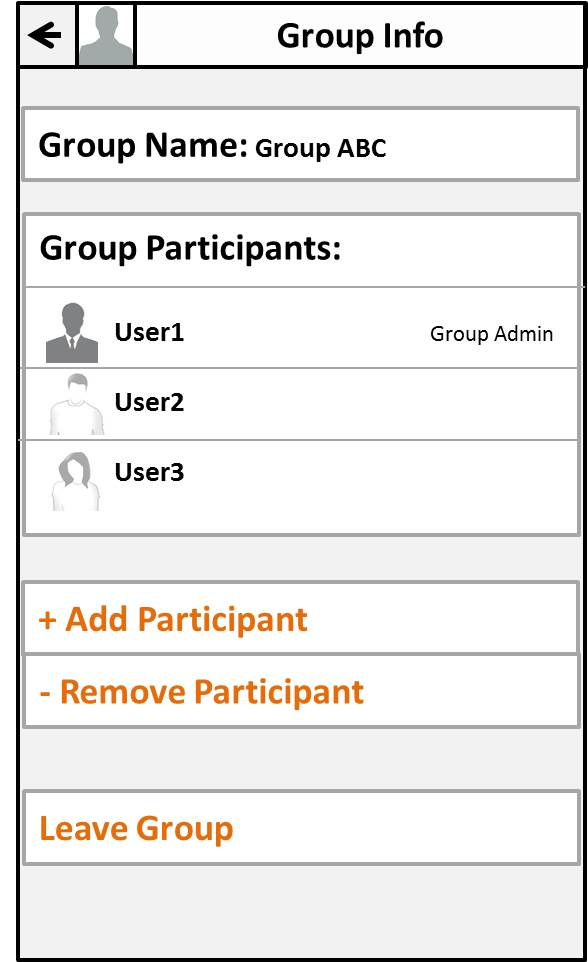
\includegraphics[width=2in]{./images/SettingF.jpg}
\caption[Sample Group Chat Information Screen]{This diagram shows how the group chat information interface is intended to look.}
\label{cd-group-chat-settings-interface}
\end{figure}

\paragraph{Colours}
\begin{itemize}
\item	In order to maintain consistency of design, the same colours chosen to represent the background throughout the application will be used for the user interface for group chats.
\item	The colour of the text will remain standard. Text that is important or selectable will be highlighted with a colour to make it noticeable - the default colour is orange. 	\\
\end{itemize}

\paragraph{Font}
\begin{itemize}
\item	In order to maintain consistency of design, the font size for each message will be the same as the chosen font size for individual chats.
\item The spacing between text will be adjusted to accommodate reading best.\\
\end{itemize}

\paragraph{Space}
\begin{itemize}
\item	Moving the group name and picture to appear in the same panel as the "Back" button will allow for more chat space thus more space and less cluttered interface.
\end{itemize}

\paragraph{Icons}
\begin{itemize}
\item	"+" Will be used to symbolize adding a participant to the group.  
\item "-" Will be used to symbolize removing a participant from the group.
\item The "Back" button will be replaced by a plain standard arrow to symbolize the "Back" option.  
\end{itemize}

\paragraph{Options Possible}
\begin{itemize}
\item	Add Participants: Selecting this option will open the contacts page where one can select contacts to add to the group.
\item 	Remove Participants: Selecting this option will open the list of participants in the group where one can select contacts to remove from the group.
\item Leave Group: Selecting this option will cause the user to leave the group and no longer receive messages from the specific group.\\
\end{itemize}



\subsubsection{Group Chat Creation}
\begin{figure}[H]
\centering
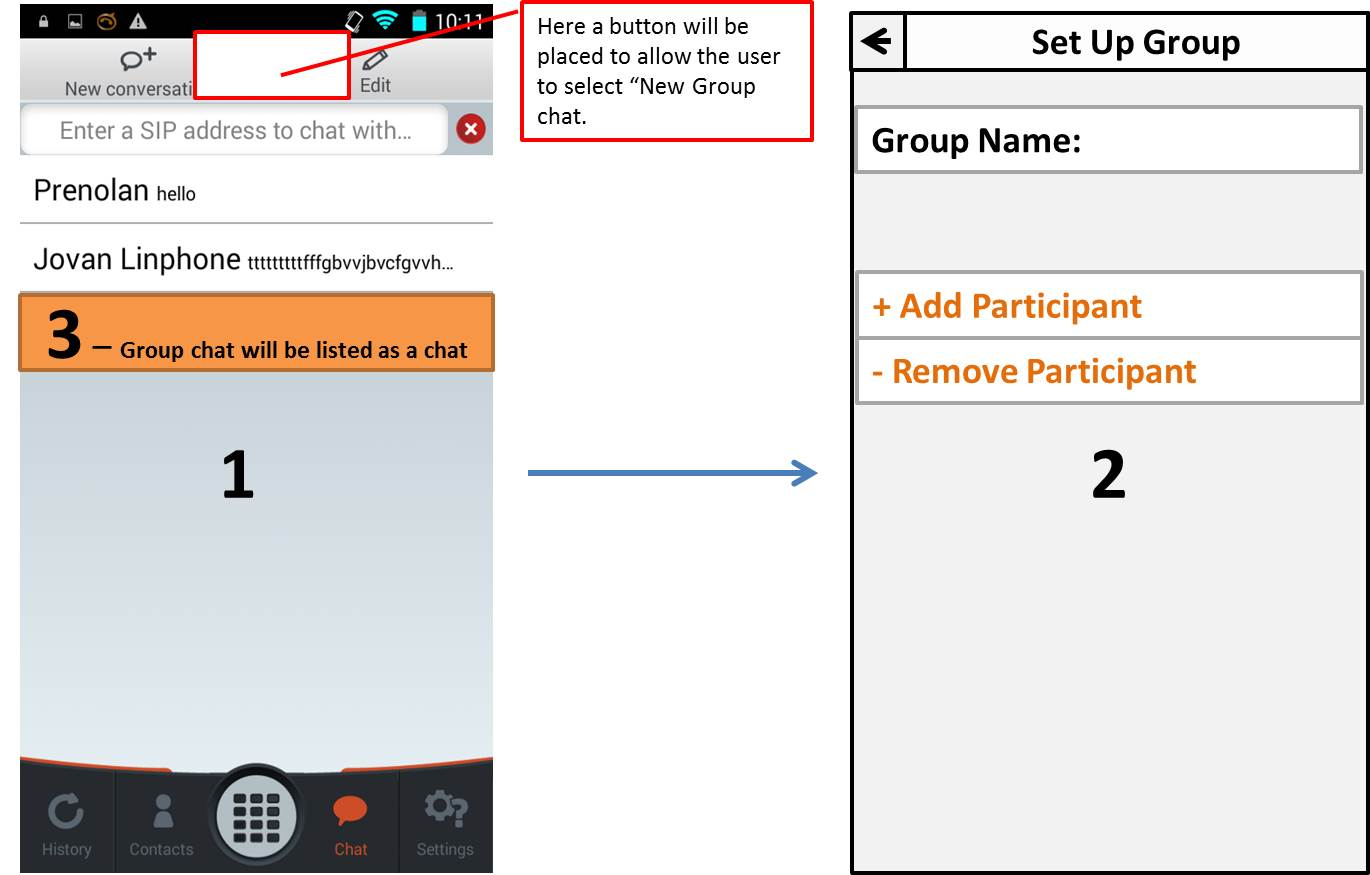
\includegraphics[width=3in]{./images/CG.jpg}
\caption[Create Group Chat]{This diagram shows how the group chat will be created.}
\label{cd-cg}
\end{figure}

\paragraph{Colours}
\begin{itemize}
\item	In order to maintain consistency of design, the same colours chosen to represent the background throughout the application will be used for the user interface for group chat creation option.
\item	The colour of the text will remain standard. Text that is important or selectable will be highlighted with a colour to make it noticeable - the default colour is orange. 	\\
\end{itemize}

\paragraph{Font}
\begin{itemize}
\item	In order to maintain consistency of design, the font size for each message will be the same as the chosen font size for the rest of the application.
\item The spacing between text will be adjusted to accommodate best reading.\\
\end{itemize}

\paragraph{Icons}
\begin{itemize}
\item	"+" Will be used to symbolize adding a participant to the group.  
\item "-" Will be used to symbolize removing a participant from the group.
\item The "Back" button will be replaced by a plain standard arrow to symbolize the "Back" option. 
\item A paper clip represents attaching a media file, in this case a profile picture.  
\end{itemize}

\paragraph{Options Possible}
\begin{itemize}
\item Type group name.
\item Select or browse phone gallery to set a profile picture for the group.
\item	Add Participants: Selecting this option will open the contacts page where one can select contacts to add to the group.
\item 	Remove Participants: Selecting this option will open the list of participants in the group where one can select contacts to remove from the group.
\end{itemize}

\paragraph{Process}
\begin{enumerate}
\item The user will, in the "Chat" interface select the option "New Group Chat" - number 1 in the diagram.
\item The Group chat set up page will be displayed. Here the user will fill in the necessary information needed in order to create a group chat - number 2 in the diagram.
\item Finally, once the group chat has been created, the Group chat name will appear in the list of the user's chats and will be able to be selected and used - number 3 in the diagram.
\end{enumerate}




\section{Software Interactions}
This section discusses and illustrates the activities that may take place within the extension. These activities are directly related to the functional requirements discussed in the System Requirements Specification document.
\subsection{Creating A Group}
Once a user attempts to create a group, the user will be afforded options to provide parameters for the instantiation of the group chat (which members, encryption type, etc.). Should the parameters be invalid, an exception will be thrown in order to indicate why validity has been voided. If the check has been passed, the group chat is initialised via \textit{LinphoneGroupChatManager}.
\begin{figure}[H]
\centering
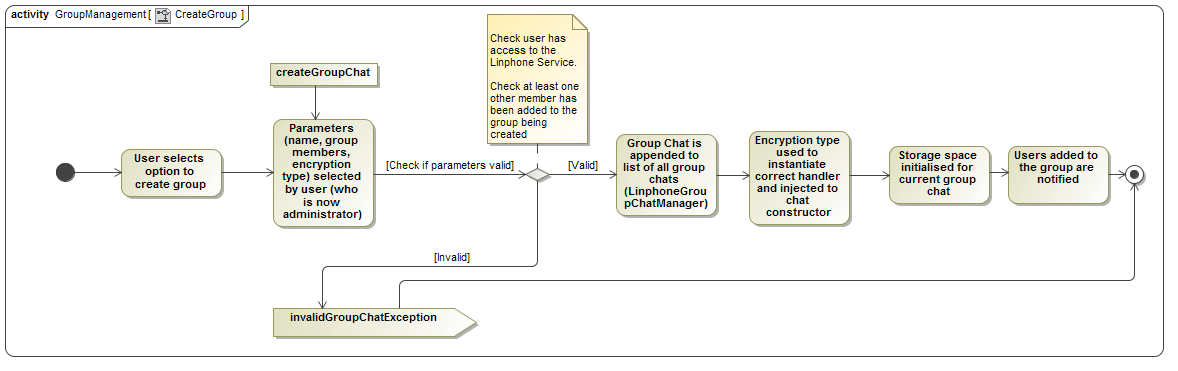
\includegraphics[width=3in]{./images/activity_create_group.png}
\caption[Create Group Activity Diagram]{This figure shows the action flow for creating a group chat.}
\label{ad-create-group}
\end{figure}
\subsection{Deleting A Group}
Once any member of a group opts to delete the group, that member is removed from the current member list of the group in order to reflect that they are no longer a part of the group to the system. Checks should be performed in post to this operation in order to delete the group entirely should no members be left or assign a new administrator should the current administrator leave.
\begin{figure}[H]
\centering
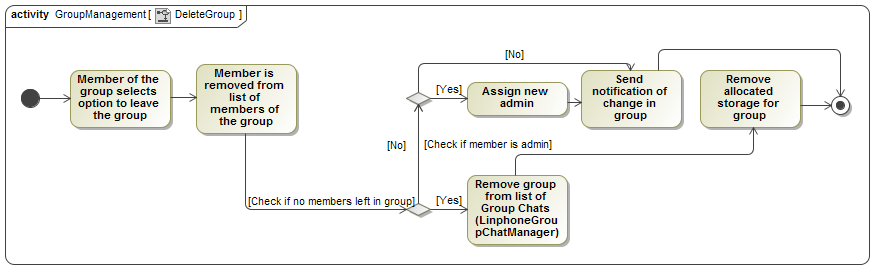
\includegraphics[width=5in]{./images/activity_delete_group.png}
\caption[Delete Group Activity Diagram]{This figure shows the action flow for deleting a group chat.}
\label{ad-delete-group}
\end{figure}
\subsection{Group Management}
Group management consists of members of a group being able to perform certain activities in order to alter the meta state of the group chat such as changing the group name, subject, or picture.
\begin{figure}[H]
\centering
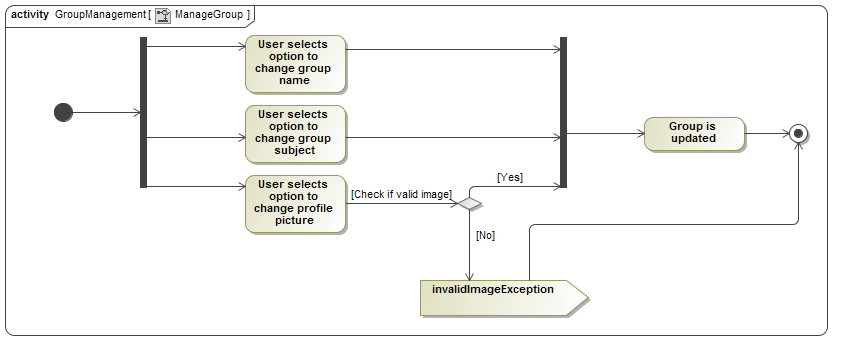
\includegraphics[width=5in]{./images/activity_manage_group.png}
\caption[Manage Group Activity Diagram]{This figure shows the action flow for managing a group chat.}
\label{ad-manage-group}
\end{figure}
\subsubsection{Adding A New Member}
Adding a member to the group chat consists of an interaction between two clients: the administrator of the group and the member to be added. The administrator initiates the process by adding the new member which is followed by the new member's client creating an instance of the existing group chat.
\begin{figure}[H]
\centering
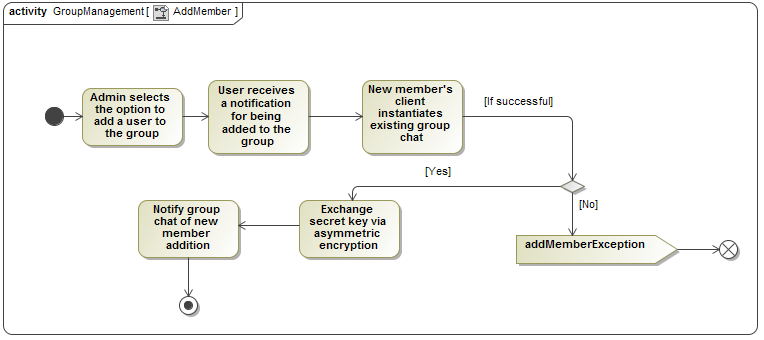
\includegraphics[width=5in]{./images/activity_add_member.png}
\caption[Add Member Activity Diagram]{This figure shows the action flow for adding a member to a group chat.}
\label{ad-add-member}
\end{figure}
\subsubsection{Removing A Member}
Removing a member from the group chat is similar to adding a member with regards to having two clients involved. The administrator initiates the process by attempting to remove a member, the member's client then handles the removal from the member list and the removal of the local group chat instance.
\begin{figure}[H]
\centering
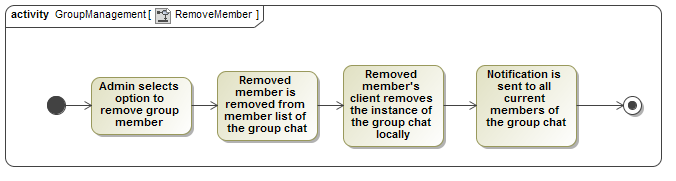
\includegraphics[width=5in]{./images/activity_remove_member.png}
\caption[Add Member Activity Diagram]{This figure shows the action flow for removing a member from a group chat.}
\label{ad-remove-member}
\end{figure}
\subsection{Sending Messages}
Each message one member sends to the group will be handled by the \textit{LinphoneGroupChatRoom} instance for that group chat. A message object will be created and sent to each of the group members using \textit{LinphoneChatRoom} instances to initiate the transaction.\\
If encryption is enabled for the group chat, the message will be encrypted using the public key of each group member before the message is sent. In the case that the current \textit{LinphoneGroupChatRoom} instance has no record of a specific member's public encryption key, the instance shall request the public key of that member before sending the message to them. Once the message has been sent to all members, the process is complete.
\begin{figure}[H]
\centering
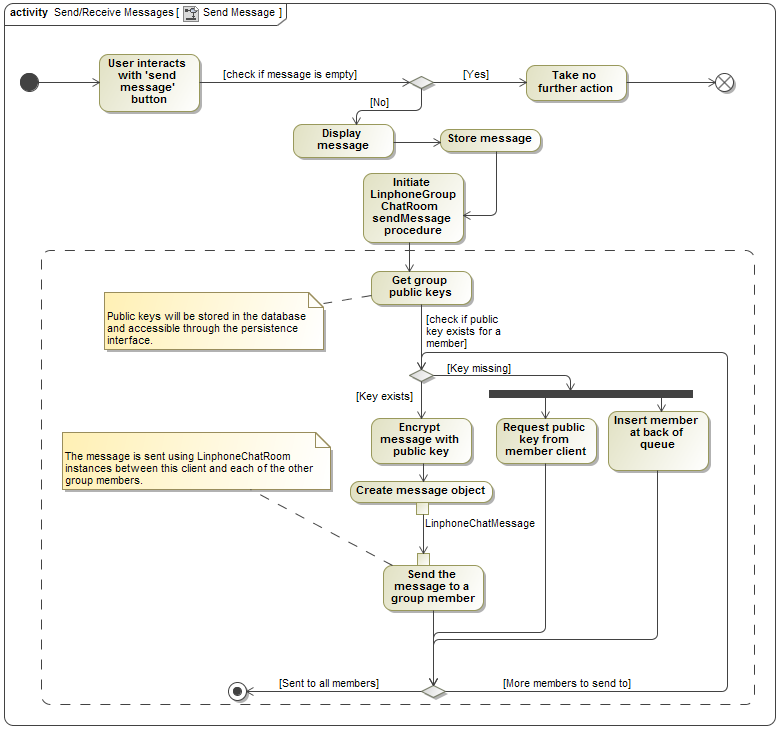
\includegraphics[width=5in]{./images/activity_send_message.png}
\caption[Send Message Activity Diagram]{This figure shows the action flow for sending a group chat message.}
\label{ad-send-message}
\end{figure}
In the case that no encryption is used, the above diagram is simplified such that a \textit{LinphoneChatMessage} object is created and sent to each member without any of the finer details present in the broken-line container.\\

During the implementation phase, the send message feature will be optimized to meet the timing and success rate requirements specified in the \textbf{Software Requirements Specification}. Sending text messages should easily meet these requirements. However, due to the nature of media files (including images and voice recordings), it is highly likely that such files will take longer to process and send --- network conditions can sometimes be unreliable and sending larger files can often fail.
\subsubsection{Recording A Voice Note}
A voice note/recording will be handled in a similar way to a text message, except that the \textit{LinphoneChatMessage} will be created using a different operation, where the sound recording will be the content of the message.\\
Before a voice note can be recorded, the application must first check if the system can provide the service of making a voice recording. If not, the process should be terminated.\\
Figure \ref{ad-voice-record} describes the above, while figure \ref{ad-send-message} describes the way in which such a message may be sent to a group. The process may also be applied to private \textit{LinphoneChatRoom} instances.
\begin{figure}[H]
\centering
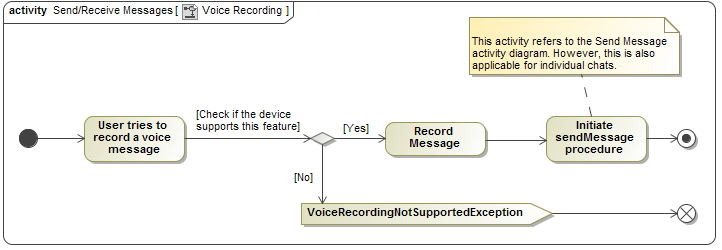
\includegraphics[width=5in]{./images/activity_voice_record.png}
\caption[Voice Recording Activity Diagram]{This diagram describes the activity flow for recording a voice note.}
\label{ad-voice-record}
\end{figure}
\subsection{Receiving Messages}
Each message received by the application will first be intercepted by a \textit{LinphoneGroupChatListener}. If the message headers contain a specific header that identifies the message as a group chat message, that message will be delegated to the \textit{LinphoneGroupChatManager}. The \textit{LinphoneGroupChatManager} will then determine which group chat the message is intended for by looking at the group chat identity specified by the message header. It will then delegate the message to the correct \textit{LinphoneGroupChatRoom} instance, which will decrypt the message before it is displayed and stored.
\begin{figure}[H]
\centering
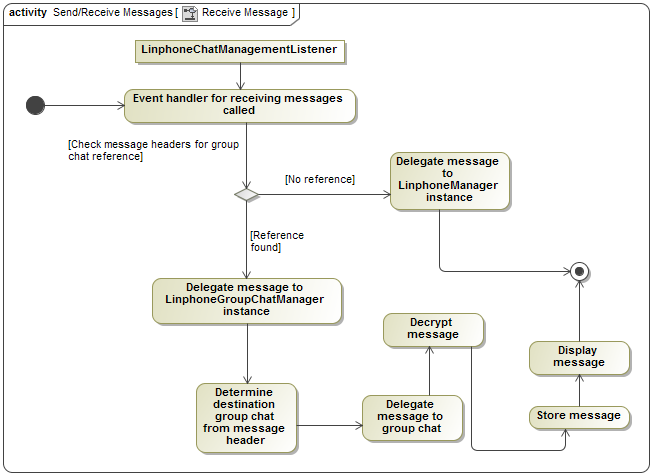
\includegraphics[width=5in]{./images/activity_receive_message.png}
\caption[Receive Message Activity Diagram]{This figure shows the action flow for sending a group chat message.}
\label{ad-receive-message}
\end{figure}
\section{Traceability Matrix}\label{section-trace-matrix}
The traceability matrix in this section shows the relationships between the design decisions in this document and the requirements specified in the \textbf{Software Requirements Specification} document.\\
For readability purposes, the matrix has been split into two halves, each with the complete list of items in this document and half the items in the \textbf{Software Requirements Specification}. Figure \ref{tbl-trace-1} shows the first half and figure \ref{tbl-trace-2} shows the second half.
\begin{figure}[H]
\centering
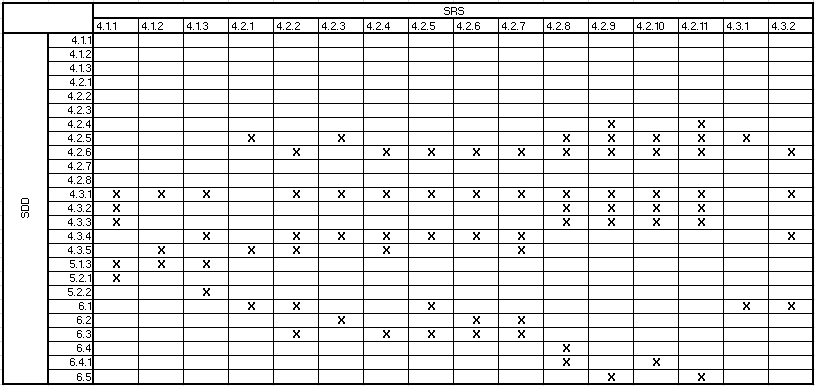
\includegraphics[width=5in]{./images/trace_matrix_1.png}
\caption[Traceability Matrix Part 1]{This table shows the first half of the traceability matrix.}
\label{tbl-trace-1}
\end{figure}
\begin{figure}[H]
\centering
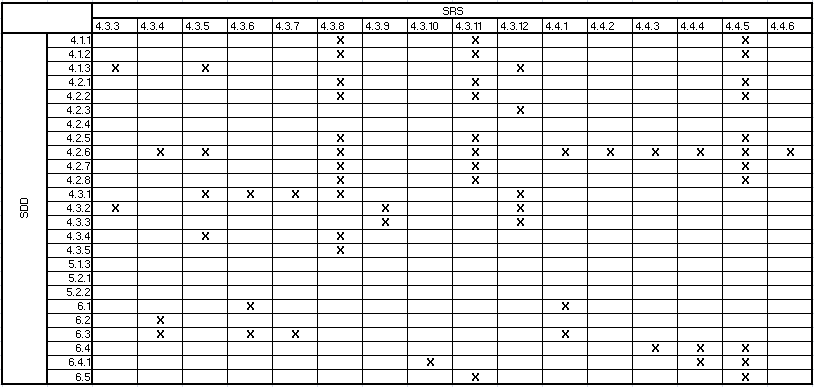
\includegraphics[width=5in]{./images/trace_matrix_2.png}
\caption[Traceability Matrix Part 1]{This table shows the second half of the traceability matrix.}
\label{tbl-trace-2}
\end{figure}
\newpage
\section{Appendix A}
\subsection{References}
\subsubsection{Liblinphone}
This document refers to the \textit{Liblinphone} core libraries. The documentation for \textit{Liblinphone} can be found at the following web page:\\
\href{http://www.linphone.org/docs/liblinphone-javadoc/}{http://www.linphone.org/docs/liblinphone-javadoc/}
\subsubsection{Android APIs}
This document makes reference to the \textit{Android} APIs. Extensive documentation for these interfaces can be found at the following link:\\
\href{http://developer.android.com/reference/packages.html}{http://developer.android.com/reference/packages.html}

\newpage
\section{Appendix B}
\listoffigures

\end{document}
